\section*{Appendix}
\label{sec:appendix}

\section{Cross-Layer Top-$k$ Index Overlap}
\label{app:topk-overlap}

To empirically validate the cross-layer redundancy of top-$k$ index selections in DSA, we compute the pairwise overlap ratio between the top-$k$ indices selected by each layer's lightning indexer.
Specifically, for every pair of layers~$(i, j)$, we measure~$|\mathcal{T}^{(i)} \cap \mathcal{T}^{(j)}| / k$ (where~$k = 2048$) averaged over 768 samples of 200K length in a calibration set.

\begin{figure}[htbp]
\centering
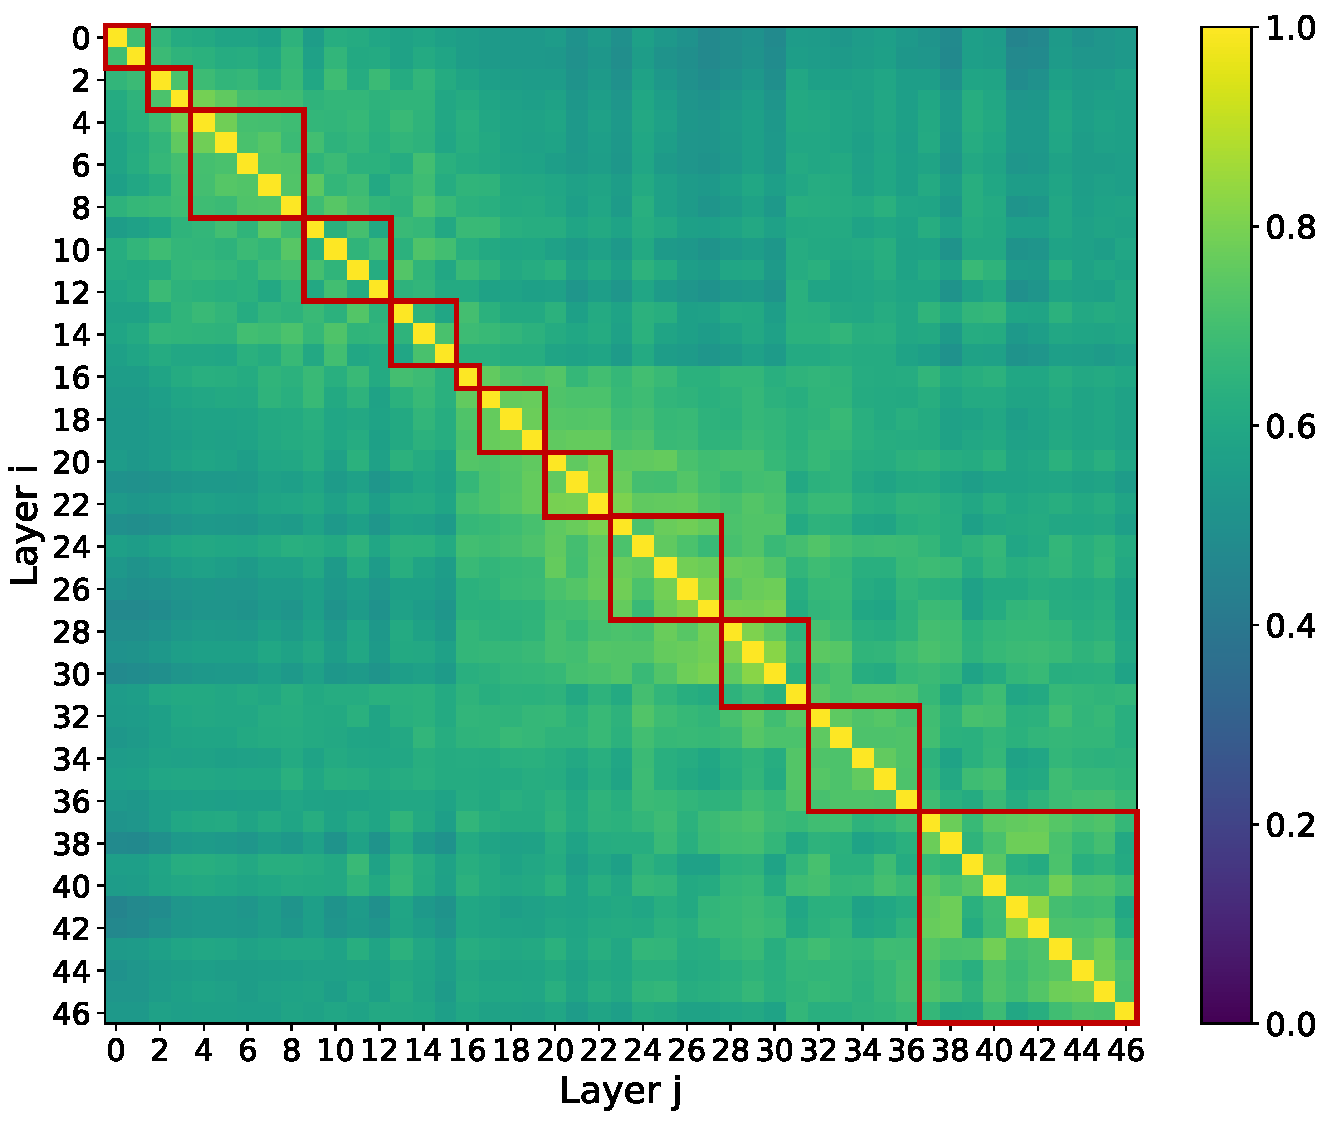
\includegraphics[width=0.7\linewidth]{figures/overlap.pdf}
\caption{Pairwise top-$k$ index overlap ratio between all layer pairs of the 30B DSA model. Shared blocks according to the greedy-searched 1/4 IndexCache pattern are \textcolor{BrickRed}{\textbf{marked}}.}
\label{fig:topk-iou-heatmap}
\end{figure}

Figure~\ref{fig:topk-iou-heatmap} visualizes this overlap as a heatmap for the 47-layer 30B DSA model, with the sharing blocks from the greedy-searched 1/4-retention pattern marked as red boxes.
Several patterns are evident:
\begin{itemize}[leftmargin=*,itemsep=2pt]
    \item \textbf{High overlap near the diagonal.} Adjacent layers exhibit overlap ratios of~0.7-1.0, confirming that consecutive layers select largely the same set of tokens.
    \item \textbf{Block structure.} The heatmap reveals distinct clusters of layers with mutually high overlap, for instance, layers~3-5, 6-8, 17-30, 31-36, etc., suggesting that the model organizes into functional blocks where token selection is internally consistent.
    \item \textbf{Uneven decay.} Overlap decreases more rapidly across block boundaries than within them, indicating that a few ``transition'' layers shift the attention focus substantially.
    \item \textbf{Early-late distinction.} The bottom-left and top-right corners of the heatmap are notably dark (overlap~$\leq 0.4$), showing that early and late layers attend to fundamentally different token subsets.
\end{itemize}

\paragraph{Greedy-searched blocks vs.\ overlap clusters.}
Comparing the red boxes (greedy-searched sharing blocks) with the natural overlap clusters reveals an informative mismatch.
While the greedy search does place~\texttt{F}~layers near some visually obvious cluster boundaries, the two partitions do \emph{not} fully coincide.
The root cause is that overlap is an \emph{aggregate} metric: it counts how many tokens are shared but not \emph{which} ones differ.
In the training-free setting, weights are frozen, so even a small set of mismatched critical tokens can perturb a layer's hidden state in ways that cascade through all downstream layers.
Early layers are especially vulnerable because their perturbations traverse the longest propagation path.

This observation also echoes our negative result with the similarity-based pattern search (Appendix~\ref{app:similarity-search}): local metrics---whether cosine similarity of attention outputs or top-$k$ index overlap---lack the discriminative power to identify the optimal sharing pattern, necessitating end-to-end evaluation.

\section{Searched Patterns}
\label{app:pattern}
Searched patterns for GLM-4.7-Flash 30B DSA:
\begin{itemize}[leftmargin=*,itemsep=2pt]
    \item Keep 1/2 `\texttt{F}'s: \texttt{FSFSFSSSSFSFFFFSFFSSFFSFFFSSFFSSFSSSSFSFFFSFSSF}
    \item Keep 1/4 `\texttt{F}'s: \texttt{FSFSFSSSSFSSSFSSFFSSFSSFSSSSFSSSFSSSSFSSSSSSSSS}
    \item Keep 1/8 `\texttt{F}'s: 
    \texttt{FSSSFSSSSSSSSFSSSFSSSSSFSSSSFSSSSSSSSFSSSSSSSSS}
\end{itemize}
Searched patterns for GLM-5:
\begin{itemize}[leftmargin=*,itemsep=2pt]
    \item Keep 1/2 `\texttt{F}'s: \texttt{FFSFSSSFSSFFFSSSFFFSFSSSSSSFFSFFSFFSSFFFFFFSFFFFFSFFSSSSSSFSFFFS\allowbreak FSSSFSFFSFFSSS}
    \item Keep 1/4 `\texttt{F}'s: \texttt{FFSFSSSFSSFSFSSSSSSSFSSSSSSFSSSFSFSSSSFFFFFSSSFFSSSFSSSSSSSSFSSS\allowbreak FSSSSSSFSFSSSS}
\end{itemize}

\section{Similarity-based Pattern Search}
\label{app:similarity-search}
We believe papers should report not only positive results but also negative (or unsuccessful) ones.
Before arriving at the greedy loss-based search described in Section~\ref{sec:method-greedy}, we explored a seemingly natural alternative: choosing the sharing pattern by directly measuring how similar the attention outputs are when an indexer is reused across layers.
Although this approach is theoretically motivated and computationally cheaper than the greedy search, it ultimately proved insufficient as a proxy for downstream quality.
We describe it here for completeness and to provide insight into why the loss-based search is necessary.

\paragraph{Constructing the similarity matrix.}
Given a DSA model with~$N$ layers, we perform $N$ single forward passes over a calibration set and, for each layer pair~$(i, j)$ with~$i > j$, compute the cosine similarity between:
\begin{enumerate}[leftmargin=*,itemsep=1pt]
    \item the core attention output at layer~$i$ when using layer~$i$'s \emph{own} indexer (i.e., the original model), and
    \item the core attention output at layer~$i$ when \emph{reusing} layer~$j$'s indexer (i.e., as if layer~$i$ were an~\texttt{S}~layer sharing from layer~$j$).
\end{enumerate}
This yields an $N \times N$ lower-triangular similarity matrix~$\mathbf{S}$, where $S_{i,j}$ quantifies how well layer~$j$'s index can serve as a proxy for layer~$i$'s own index.
Intuitively, if $S_{i,j}$ is close to~1, then layer~$i$ can safely skip its own indexer computation and reuse the index from layer~$j$ with minimal distortion to its attention output.

\paragraph{Dynamic programming formulation.}
Given the similarity matrix~$\mathbf{S}$ and a target number of~\texttt{F}~layers~$M$ (equivalently, $N - M$~\texttt{S}~layers), we seek the pattern~$\mathbf{c}^*$ that maximizes the total similarity:
\begin{equation}
    \mathbf{c}^* = \arg\max_{\mathbf{c}:\, |\{i : c_i = \texttt{F}\}| = M} \;\sum_{\ell:\, c_\ell = \texttt{S}} S_{\ell,\, \mathrm{src}(\ell)}
\end{equation}
where $\mathrm{src}(\ell)$ denotes the most recent preceding~\texttt{F}~layer from which layer~$\ell$ inherits its index (i.e., $\mathrm{src}(\ell) = \max\{j < \ell : c_j = \texttt{F}\}$).

This can be solved exactly via dynamic programming.
Let $\mathrm{dp}[i][k]$ denote the maximum cumulative similarity achievable for layers~$1, \ldots, i$ using exactly~$k$~\texttt{F}~layers, with layer~$i$ itself being an~\texttt{F}~layer.
The transition considers all possible previous~\texttt{F}~layers:
\begin{equation}
    \mathrm{dp}[i][k] = \max_{j < i,\; c_j = \texttt{F}} \left\{ \mathrm{dp}[j][k{-}1] + \sum_{m=j+1}^{i-1} S_{m,j} \right\}
\end{equation}
where the summation accounts for all~\texttt{S}~layers between~$j$ and~$i$, each reusing layer~$j$'s index.
We recover the optimal pattern by backtracking through the DP table.

\begin{table}[t]
\centering
\caption{%
    Evaluation results of training-free \emph{similarity-based} searched pattern.
}
\label{tab:sim}
\resizebox{0.7\textwidth}{!}{%
\begin{tabular}{l cccc}
\toprule
& \textbf{Avg} & \textbf{MRCR v2} & \textbf{GraphWalks} & \textbf{RULER} \\
\midrule
Original DSA & \textbf{54.0} & \textbf{24.5} & \textbf{49.6} & \textbf{87.9}  \\
\midrule
\rowcolor{mygray}1/2 Unif. IndexCache & 50.7 & 22.0 & 46.6 & 83.6 \\
\quad+Searched pattern & 49.8 & 22.9 & 43.5 & 82.9 \\
\bottomrule
\end{tabular}%
}
\end{table}

\paragraph{Result: similarity-optimal patterns perform comparably to uniform interleaving on downstream tasks.}
Like uniform interleaving, DP-searched patterns exhibit the same significant quality degradation relative to the original DSA model, as shown in Table~\ref{tab:sim}.
In other words, despite explicitly optimizing for maximal cross-layer similarity, the resulting patterns offer no meaningful advantage over the na\"{\i}ve uniform baseline.
In contrast, the greedy loss-based search (Section~\ref{sec:method-greedy}) produces patterns that \emph{substantially} outperform both uniform and similarity-optimal patterns, especially at aggressive retention ratios.

\paragraph{Why similarity fails as a proxy.}
The fundamental issue is that per-layer output similarity is a \emph{local} metric: it measures how well a single layer's attention output is preserved in isolation, without accounting for how small perturbations propagate across the remaining layers.
Two layers may have nearly identical attention outputs ($S_{i,j} \approx 1$) yet differ in subtle ways that matter for downstream quality: for instance, the reused index may miss a small number of critical tokens whose importance only becomes apparent in later layers' reasoning steps.
These subtle mismatches accumulate through the layers, leading to non-negligible final quality degradation that a layer-local similarity score cannot predict.

The greedy loss-based search avoids this pitfall by directly optimizing a \emph{global} metric, i.e., the LM loss, which captures the end-to-end effect of each sharing decision on the model's output distribution.
This allows it to identify ``critical'' layers (those whose indexers must be retained to avoid cascading errors) that the similarity-based approach treats as interchangeable with their neighbors.

\section{Evaluation Setup}
\label{app:eval}
All benchmarks are evaluated with temperature~1.0, top-$p$~=~0.95, and top-$k$~=~40. For long-context tasks, we set a total context window of 200K tokens with 32K reserved for the output. For general \& reasoning tasks, we allow a maximum output length of 64K tokens.
On MRCR~v2, we report the average score across 2-, 4-, and 8-needle settings.
On GraphWalks, we report the average score over the Parent-type and BFS-type problems.
On RULER, we report scores on all instances with context lengths ranging from 4K to 128K.
For MRCR~v2 and GraphWalks, we include only instances whose input length fits within the effective input budget (200K$-$32K$=$168K tokens).
For LongBench~v2, RULER, and AA-LCR, we include all instances and apply middle truncation to those exceeding 168K tokens.